%---------------------------------------------------------------------
%
% Chapter 1: Introduction
%
%---------------------------------------------------------------------
%
% ChapIntroduction.tex
% Copyright 2015 Dr. Francisco J. Pulido
%
% This file belongs to the PhD titled "New Techniques and Algorithms for Multiobjective and Lexicographic Goal-Based Shortest Path Problems", distributed under the Creative Commons Licence Attribution-NonCommercial-NoDerivs 3.0, available in http://creativecommons.org/licenses/by-nc-nd/3.0/. The complete PhD dissertation is freely accessible from http://www.lcc.uma.es/~francis/
%
% This thesis has been written adapting the TeXiS template, a LaTeX template for writting thesis and other documents. The complete TeXiS package can be obtained from http://gaia.fdi.ucm.es/projects/texis/. TeXis is distributed under the same conditions of the LaTeX Project Public License (http://www.latex-project.org/lppl.txt). The complete license is available in http://creativecommons.org/licenses/by-sa/3.0/legalcode
%
%---------------------------------------------------------------------

\chapter{Introduction}
\label{chapIntroduction}


\begin{FraseCelebre}
\begin{Frase}
Research is what I'm doing when I don't know what I'm doing
\end{Frase}
\begin{Fuente}
Wernher von Braun (1912-1977)
\end{Fuente}
\end{FraseCelebre}
%
%\begin{resumen}
%...
%\end{resumen}

This doctoral dissertation falls within the scope of the Artificial Intelligence (AI) and Operations Research (OR) fields. Shortest Path Problems (SPP) are one of the oldest and most extensively studied problems in both fields, which consists in finding the shortest path between two given nodes in a graph such that the sum of the weights of its constituent arcs is minimized. The SPP arises naturally in real life, e.g. planning the route path in a road trip, or navigating a mobile robot to avoid obstacles, and can be also used to solve optimally puzzle games like Rubik's cube \citep{Korf1997} or the twenty-four puzzle \citep{Korf1996}.

The Multicriteria Search Problem (MSP), or Multiobjective Shortest Path Problem, is the natural extension to the SPP whenever more than one criterion is considered. The MSP is computationally harder than the single objective one. The number of label expansions can grow exponentially with solution depth, even for the two objective case \citep{hansen1979}. With the assumption of bounded integer costs and a fixed number of objectives the problem becomes tractable for polynomially sized graphs, but still harder than single objective search (e.g. see \citep{Mandow2009,Muller-Hannemann2006}).

Recent experiments on problems like bicriteria route planning have revealed that time, rather than space, is the practical limiting factor in the calculation of the full set of efficient solutions in exact algorithms in Multicriteria Search \citep{Machuca2011b, Machuca2009}. In this thesis we address this problem from the point of view of Goal Programming (GP), which has proven to be a very effective model of decision maker's preferences over multicriteria decision making (MCDM) problems. Goal Programming is a general paradigm which claims that a decision problem can be expressed through a set of goals defined by the decision maker, rather than through the optimization of a set of objectives. Roughly speaking, a goal defines a degree of satisfaction of a given criteria that is deemed satisfactory or acceptable by the decision maker. One of the most commonly used schemes to express goal-based preferences is the lexicographic method of grouping criteria by pre-emptive importance \citep{Charnes1977,Romero1991}.

Our starting hypothesis is that in those cases where user preferences can be initially bounded by a set of goals, specially designed search algorithms could perform more efficiently than searching for the full Pareto frontier. The main goals of this thesis are to explore this hypothesis, and to improve the performance of current multiobjective search algorithms. More precisely, we explore new algorithmic contributions to the MSP with lexicographic goal-based preferences, and also a new technique to speed up multicriteria search algorithms based on labeling techniques.    

Section \ref{ChapIntroduction:sec:motivation} introduces the motivation and significance of this work for the AI and OR fields. Section \ref{ChapIntroduction:sec:orientation} presents our scope and orientation. The goals and contributions of this thesis are enumerated in Sections \ref{ChapIntroduction:sec:objectives} and \ref{ChapIntroduction:sec:contributions}, respectively. Related publications of this research work are shown in Section \ref{ChapIntroduction:sec:publications}. Finally, Section \ref{ChapIntroduction:sec:outline} outlines the structure of this thesis.

%-------------------------------------------------------------------
\section{Motivation}
\label{ChapIntroduction:sec:motivation}
%-------------------------------------------------------------------

The Shortest Path Problem is a recurrent problem in the AI and OR literature. \citet{dijkstra1959} proposed the first algorithm to find the minimal cost route between two nodes in a graph. The A$^*$ algorithm \citep{Hart1968} is an important algorithmic reference that exploits specific problem knowledge (the so-called heuristic function in the AI community) to guide the search and improve its efficiency. This problem knowledge is in the form of a distance or cost estimate.

Real life decision problems frequently involve the consideration of multiple criteria simultaneously. For example, Figure \ref{ChapIntroduction:fig:sample-app} shows three car routes from M\'{a}laga to Valencia (both in Spain) suggested by a sample web application devoted to road route planning. Assume we are concerned with the minimization of three different criteria in this problem: travel cost, time and distance. Route \ref{ChapIntroduction:fig:sample-app-1} is the fastest and shortest route and Route \ref{ChapIntroduction:fig:sample-app-3} is the cheapest. Whenever there are no other preferences defined, we say that both routes are \emph{efficient solutions} to this problem, i.e. these solutions represent an optimal trade-off between the criteria. These are extreme efficient solutions, but there might well be other interesting trade-offs. The set of all solutions such that none of the objectives can be improved without worsening at least one of the others, is called the Pareto set or Pareto frontier, and they are call efficient or non-dominated solutions.

\begin{figure}
    \begin{center}
      \subfigure[Route 1]{\label{ChapIntroduction:fig:sample-app-1}
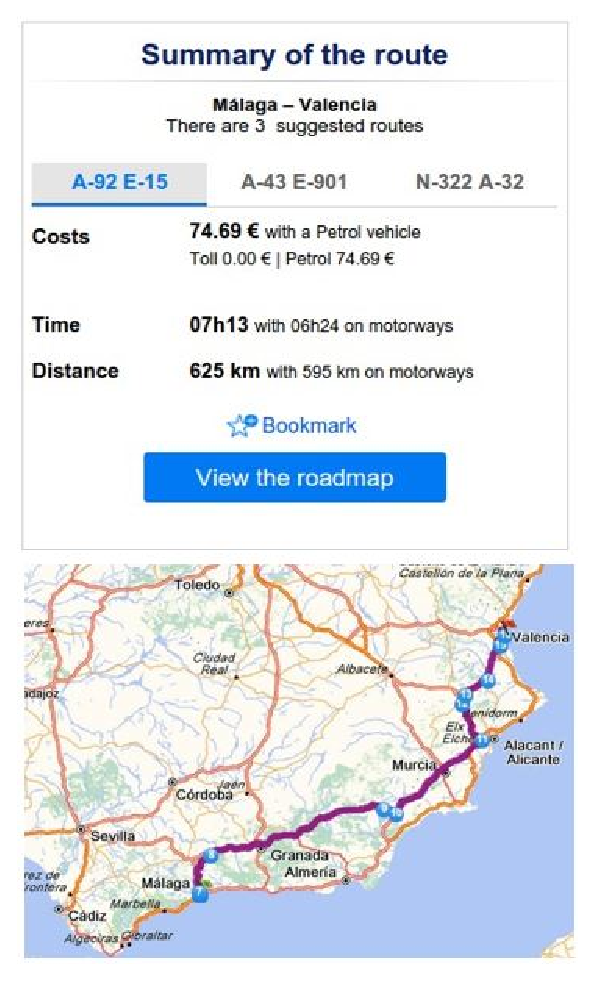
\includegraphics[width=0.3\textwidth]{Images/Chapter1/sample-app-1}
        }
        \subfigure[Route 2]{ \label{ChapIntroduction:fig:sample-app-2}
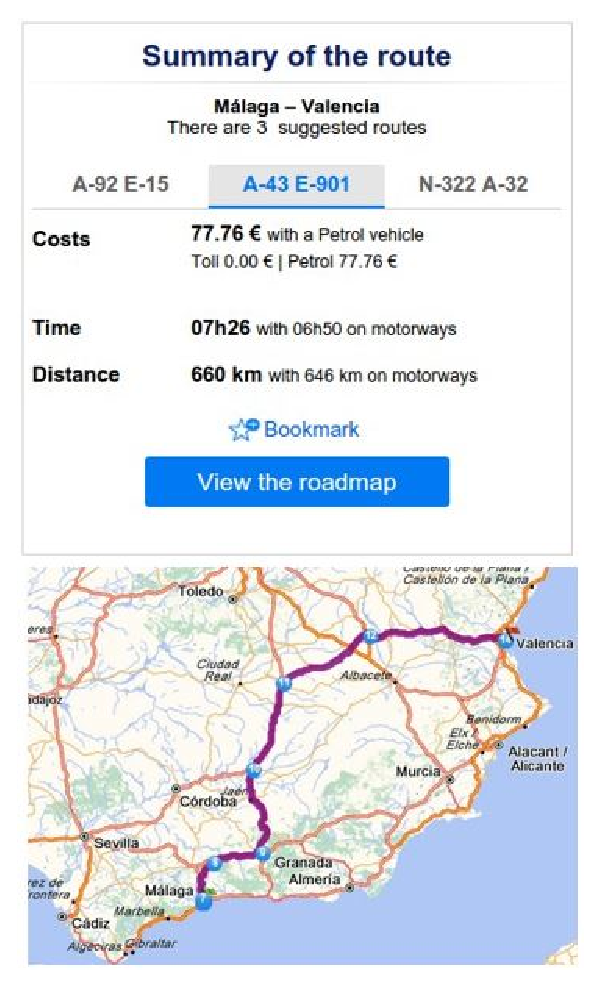
\includegraphics[width=0.3\textwidth]{Images/Chapter1/sample-app-2}
        }
       \subfigure[Route 3]{\label{ChapIntroduction:fig:sample-app-3}
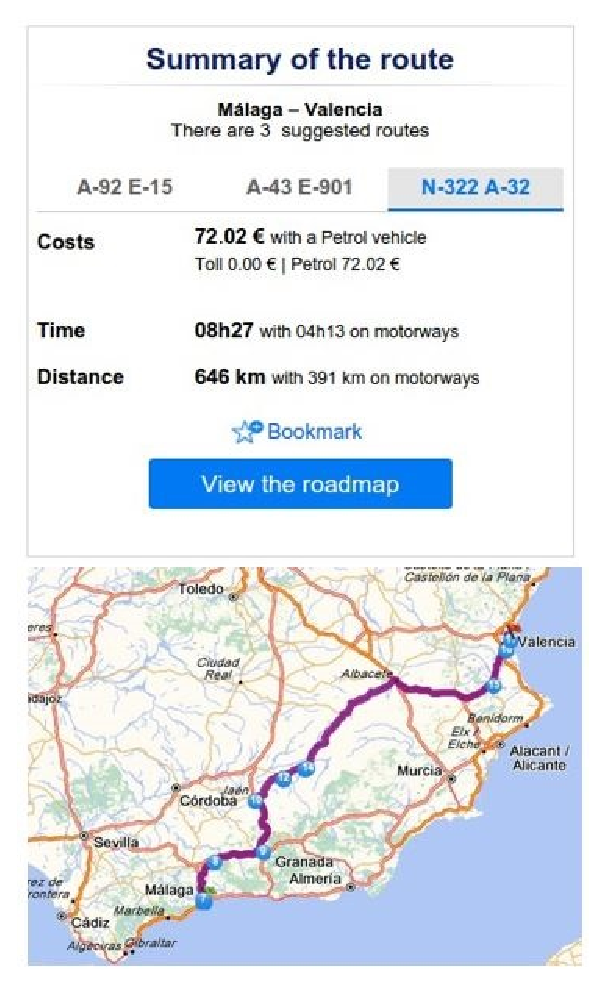
\includegraphics[width=0.3\textwidth]{Images/Chapter1/sample-app-3}
        }
    \end{center}
    \vspace{-0.25in} 
    \caption{
      Screenshots from a sample route planning web application, showing alternative routes from M\'{a}laga (Spain) to Valencia (Spain). \copyright \ \url{www.viamichelin.com}
    }
    \label{ChapIntroduction:fig:sample-app}
\end{figure}

Among all feasible routes in our example only a subset can be considered non-dominated in terms of all objectives. Thus, route \ref{ChapIntroduction:fig:sample-app-2} is called a dominated solution, since there is another route, route \ref{ChapIntroduction:fig:sample-app-1}, that is lower in all objectives. However, the calculation of the Pareto set is typically a hard problem, hence, we consider the application of Goal Programming (GP) to model the decision maker's preferences and establish a set of goals that  restrict the set of solutions to those ones which satisfy those goals, or which minimize the deviation from the goals if they can not be satisfied. Thus, in our example, a user of the road route planner can define their expectations of the maximum economic cost, time and distance for the trip.

In order to deal with the problem described above, two different alternatives can be followed. In the first one, a full Multicriteria Search algorithm can return the full Pareto set of solutions to the problem. This set can then be used to determine the subset of solutions that satisfy the goals, or in case the goals can not be fully satisfied, the subset which minimizes the deviation from those goals according to a given definition of distance. For this alternative, we consider \namoa, which is currently the most efficient exact algorithm to calculate the Pareto frontier.

The second alternative to deal with the MSP with goal-based preferences concentrates the search effort on the subset of Pareto optimal solutions that satisfy the goals, discarding those paths that will not lead to efficient solutions according to the goals. Notice that we shall always seek for efficient or non-dominated solutions for the problem, regardless whether the goals can be satisfied or not. This is not the case of Goal Programming in general, that allows non-dominated solutions to the problem. 

For the second alternative, we introduce \lexgo, a best-first Multicriteria Search algorithm that is also exact and efficient when provided with consistent lower bounds. 

Finally, this thesis is also devoted to improve the time performance of exact multicriteria search algorithms with consistent lower bounds and to do so, a new dimensionality reduction technique is introduced. This technique allows discarding non-dominated paths with a dramatic decreased number of dominance checks against permanent labels. Its application to \namoa \ and \lexgo \ leads to the introduction of two new algorithms, \namoate \ and \lexgote. Their effectiveness is also studied from formal and empirical points of view against traditional pruning or discarding.  

%-------------------------------------------------------------------
\section{Scope and Orientation}
\label{ChapIntroduction:sec:orientation}
%-------------------------------------------------------------------

We summarize the boundaries of this doctoral dissertation with the following terms:

\begin{description}
	
	\item[Multicriteria Search with lower bounds.] The Shortest Path Problem consists in finding the shortest path between two nodes in a graph. The natural extension when considering multiple conflicting criteria is the Multicriteria Search Problem. We consider the $A^*$ algorithm as a reference in the solution of this problem and, therefore, analyze multicriteria search algorithms whose
performance can improve with the use of lower bounds or distance estimates to restrict the number of label expansions.
	
	\item[Additive costs.] Arcs in the graph are labeled with a magnitude for each criterion, or cost, under consideration. In the MSP, the arcs in the graph represent the costs of navigating from the source to the destination node. The cost of the route in the graph to be minimized corresponds to the sum of the costs vectors of its component arcs. 
	
	\item[Pareto optimality.] When multiple criteria are considered, the concept of minimum no longer applies, and is usually replaced by that of Pareto optimality. Pareto optimal solutions are defined as those that cannot be improved according to one objective without worsening at least one of the others.
	
	\item[Label-setting multicriteria search algorithms.] 
Best-first algorithms are classified in the OR literature as label-setting or label-correcting. The former explores only optimal paths in the graph, and therefore set permanent labels for each scanned node. The latter may also explore suboptimal paths and therefore may establish temporary labels for scanned nodes. When algorithms A$^*$ or \namoa \ use consistent lower bounds as cost estimates, they behave as label-setting algorithms. That will also be the case for the algorithms analyzed in this thesis.
	
	\item[Pre-emptive and weighted preferences.] 
Goal Programming models preferences given by a decision maker for a multicriteria problem. We focus on the technique where the criteria are grouped in priority levels sorted in order of decreasing pre-emptive importance. Furthermore, a level comprises a set of one or more attributes. We define targets for each attribute and weights to establish the importance of the criteria within the level. 

	\item[Theoretical proofs of correctness.] We contribute in this thesis several new algorithms. Formal proofs of their admissibility and efficiency are provided. These are complemented with empirical analyses of the algorithms.

\end{description}

%-------------------------------------------------------------------
\section{Research Goals}
\label{ChapIntroduction:sec:objectives}
%-------------------------------------------------------------------

The main goals of this doctoral dissertation can be outlined as follows:

\begin{enumerate}
	\item \textbf{Address the Multicriteria Search Problem with goal-based preferences.} The first goal of this thesis is the description of the Multicriteria Search Problem and specifically, the Multicriteria Search Problem with Preferences Based on Goals. We will describe the two considered approaches to deal with such a problem in detail. 

	\item \textbf{Devise a new algorithm to cope with lexicographic goal-based preferences.} The principle of optimality holds for Multiobjective Shortest Path Problems, but regrettably does not hold for lexicographic goal-based preferences. In order to approach the MSP with a specifically designed goal-based algorithm, we concentrate our efforts to devise a new algorithm  based on a label selection policy.  

	\item \textbf{Prove formally the correctness and efficiency of this new algorithm.} Another goal of this thesis is to complement the defined algorithm with formal analyses of its correctness as well as its efficiency over an optimal algorithm that performs a full Multiobjective Search (\namoa).	

	\item \textbf{Study possible improvements to multiobjective shortest path algorithms.} Our efforts will also be focused on the improvement of multiobjective shortest path algorithms in general. More specifically, we aim to introduce a new dimensionality reduction technique to improve the runtime performance of label-setting multiobjective shortest path algorithms with consistent lower bounds.

	\item \textbf{Prove formally the correctness of the dimensionality reduction technique.} We will formally develop the application of the dimensionality reduction technique to the new defined algorithm based on goal preferences, as well as the application to \namoa. In particular, we will prove theoretically the correctness of both algorithms when employing the dimensionality reduction technique.

	\item \textbf{Perform an empirical evaluation of all the algorithmic alternatives.} Finally, the last goal of this dissertation is to provide an extensive evaluation of all the proposed algorithms. We will employ test beds over randomly generated and realistic scenarios.
\end{enumerate}

%-------------------------------------------------------------------
\section{Contributions}
\label{ChapIntroduction:sec:contributions}
%-------------------------------------------------------------------
 
The contributions of this thesis are enumerated as follows: 

\begin{enumerate}
	\item \textbf{Description of the Goal-Based Multicriteria Graph Search Problem.} In the first place, we outline the Goal Programming technique within the Multicriteria Decision Making discipline. We also outline the Multicriteria Graph Search within the Multiobjective Optimization Problem, and given that framework, we will describe and define formally the Goal-Based Multicriteria Graph Search problem and the different algorithmic approaches to deal with it.  

	\item \textbf{A new Multicriteria Search algorithm for the MSP.} We introduce \lexgo \ (Lexicographic Goals A$^*$), a new exact label-setting algorithm for Multicriteria Search problems with goal-based preferences. \lexgo \ returns the subset of non-dominated optimal paths that satisfy a set of lexicographic goals, or the subset that minimizes deviation from goals if these cannot be fully satisfied.

	\item \textbf{Formal characterization of the admissibility and efficiency of \lexgo.} We prove theoretically the admissibility of \lexgo, i.e. the algorithm is exact and returns the whole set of solutions to the problem, as well as its efficiency, i.e. the number of labels scanned by the algorithm decreases with better (more informed) lower bounds, over the full Multicriteria Search.

	\item \textbf{Introduction of \emph{t-discarding}.} We introduce a new dimensionality reduction technique called \emph{t-discarding}. This technique can be applied to the processes of pruning and filtering in order to reduce in one dimension the size of the vectors considered to discard new alternatives. Thus, we will reduce the amount of time needed to check dominance against closed vectors and therefore, the time requirements of the algorithms.

	\item \textbf{Formal characterization of the t-discarding technique.} We apply t-discarding to \namoa \ and \lexgo, introduce new algorithms \namoate \ and \lexgote, show their correctness, evaluate their effectiveness, and analyze their performance.  

	\item \textbf{Empirical evaluation of the new algorithmic contributions.} Two main scenarios are used to test the effectiveness of our devised algorithms, random grids and realistic road maps problems. We present dramatic reduction in time requirements for three-objective, four-objective and five-objective search problems over random grids. To the best of our knowledge, the results reported over road maps problems represent the largest three-objective search problems solved to date. 		
\end{enumerate}

%-------------------------------------------------------------------
\section{Related Publications}
\label{ChapIntroduction:sec:publications}
%-------------------------------------------------------------------

Contributions of this thesis has been presented in international peer-reviewed journals and conferences.

\begin{itemize}

    \item \textbf{\large Journals:}
\par
Pulido, F. J., Mandow, L., \& P\'{e}rez de la Cruz, J. (2014). Multiobjective shortest path problems with lexicographic goal-based preferences. European Journal of Operational Research, 239(1), 89-101. doi:10.1016/j.ejor.2014.05.008
\par 
Pulido, F. J., Mandow, L., \& P\'{e}rez de la Cruz, J. (2015). Dimensionality reduction in multiobjective shortest path search. Computers \& Operations Research. Volume 64, 60-70. doi:10.1016/j.cor.2015.05.007
%
    \item \textbf{\large Conferences:}
\par
Mandow, L., Pulido, F. J., \& P\'{e}rez de la Cruz, J. L. (2013). Searching Graphs with Lexicographic Goal Preferences. In 22nd International Conference on Multiple Criteria Decision Making - MCDM 2013.

\end{itemize}

%-------------------------------------------------------------------
\section{Outline}
\label{ChapIntroduction:sec:outline}
%-------------------------------------------------------------------

This doctoral dissertation is structured in eight chapters grouped in three parts. The first part is devoted to present the motivation of this thesis, its foundations and previous work, and comprises this introductory chapter, and Chapters \ref{chapMultiObjAlg} and \ref{chapMultiObjTestBeds}. Chapter \ref{chapMultiObjAlg} introduces the reader to the Multicriteria Search Problem with lexicographic goal-based preferences. Relevant models of decision maker's preferences are enumerated and several practical applications are described. This chapter also introduces the fundamentals of Multicriteria Search Problems, reviews different kinds of multiobjective search methods, and presents \namoa, the reference algorithm we use to evaluate our contributions under a common framework. Chapter \ref{chapMultiObjTestBeds} briefly reviews previous relevant multiobjective benchmarks. A set of good practices in the experimental evaluation of algorithms as well as the key concepts to measure the performance of Multicriteria Search are also presented. Finally, benchmarks employed in this thesis are described in detail. 

The second part of this dissertation groups the main contributions of this thesis. Chapter \ref{chapContributions} presents 
%relevant new definitions of lexicographic preferences and dominance checks, as well as 
the new algorithms \lexgo, \namoate \ and \lexgote. Chapter \ref{chapFormalAnalysis} gives a formal analysis of the algorithms devised as a result of this thesis, and presents the proofs for their properties of exactness and efficiency, i.e. it is formally proved for each algorithm in this thesis that the full set of efficient solutions is returned and the number of explored labels decreases with more informed lower bounds. Chapters \ref{chapEmpiricalAnalysisGrids} and \ref{chapEmpiricalAnalysisRoadMaps} analyze the performance of all the algorithmic alternatives over random grids and realistic road maps problems, respectively. These reveal the effectiveness of the proposed techniques.

Finally, part three summarizes the conclusions of this thesis and introduces future lines of work in Chapter \ref{ChapConclusions}.
